\section{Methods}
\subsection{Kinetic model}
The whole binding-cleavage process begins with the binding between PAM and protein. It corresponds to rule\#1 mentioned before. And as the reaction proceeds, every step of it is reversible, and its irreversibility mainly depends on the binding energy of two DNA bases.
	
Here we use the term binding probability $P_{bind}$ represent the probability of sgRNA binding with DNA, with a rough assumption that the probability of cleavage is the same for every kind of binding. In total, the probability of off-target cleavage is positively correlated with the binding probability. 

The probability $P_{bind,N}$ , representing the probability of binding at the Nth position (the last position of sgRNA) of nucleotide base, is given by:
\begin{equation}
P_{bind,N}=\frac{k_f(N)}{k_f(N)+k_b(N)}=\frac{1}{1+\gamma_N} \quad
\end{equation}
where $k$ is the reaction rate constant; $f$ represents the forward reaction; $b$ represents the backward reaction. And 
\begin{equation}
 \gamma_N=\frac{k_b(N)}{k_f(N)}
\end{equation}
So for a the whole sgRNA sequence: 
\begin{equation}
P_{bind} = \frac{1}{1+\sum_{n=1}^N\coprod_{i=1}^n \gamma_i}
\end{equation}
Consider the rate constant $k_f(i)$ and $k_b(i)$:
\begin{equation}
k_f(i)=k_0exp(-(T_{i,i+1}-F_i)),k_b(i)=k_0exp(-(T_{i,i-1}-F_i))
\end{equation}
where $F_i$ means free energy of each metastable state, $T_{i,i+1}$ means the highest free energy point on the reaction path from position i to position i + 1. Therefore, $T_{i,i+1}-F_i$ is the activation energy of forward reaction and $T_{i,i-1}-F_i$ is activation energy of the backward reaction.
\begin{equation}
\Rightarrow \gamma_i=exp(-\Delta_i), \Delta_i=T_{i,i+1}-T_{i,i-1}
\end{equation}
\begin{equation}
\begin{aligned}
\Rightarrow P_{bind} = \frac{1}{1+\sum_{n=1}^N\coprod_{i=1}^n \gamma_i}=\frac{1}{1+\sum_{n=1}^N\coprod_{i=1}^n exp(-\Delta_i)}\\=\frac{1}{1+\sum_{n=1}^N exp(-\sum_{i=1}^n\Delta_i)}
\end{aligned}
\end{equation}
We define $$\Delta T_n=\sum_{i=1}^n\Delta_i$$
so
\begin{equation} 
P_{bind} =\frac{1}{1+\sum_{n=1}^N exp(-\Delta T_n)}
\end{equation}
	
From the above, it is clear that the binding probability depends only on the state transition energy, not on the free energy of metastable states. If we assume there is one dominant bias $\Delta T_{n^*}$, then this equation can be approximated as:
\begin{equation}
 P_{bind} \approx \frac{1}{1+exp(-\Delta T_{n^*})}
\end{equation}

As figure shows, we analyze the energy change of every process:\newline
$\left\{
\begin{tabular}{l}
for the PAM position (i = 0) we have $\Delta_0=\Delta PAM$\\
for a partial R-loop we have $\Delta_i = \Delta_M$ if matched and $\Delta_i = -\Delta_U$ mismatched\\
\end{tabular}
\right.$

\begin{equation}
\Delta {T_n} = {\Delta _{PAM}} + {n_M}{\Delta _M} - (n - {n_M}){\Delta _U} - {\delta _{n,N}}{\Delta _{clv}};\:n = 0...N
\end{equation}
where $n_M$ is the number of matches, $\Delta _{clv}$ is the energy change of cleavage after the process of binding is finished.\\
$\delta_{n,N}$ represents the Kronecker delta:
$\delta_{n,N}$=$\left\{\begin{array}{l}1, n=N;\\
0, n\neq N.
\end{array}
\right.$

For PAM independent systems (such as Cas13a), we instead use:
\begin{equation}
\Delta {T_n} = {n_M}{\Delta _M} - (n - {n_M}){\Delta _U} - {\delta _{n,N}}{\Delta _{clv}};\:n = 0...N
\end{equation}

To sum up, the binding probability mainly relies on the free energy change, and PAM appears as a significant energy decline.

\begin{figure}[H]
	\centering
	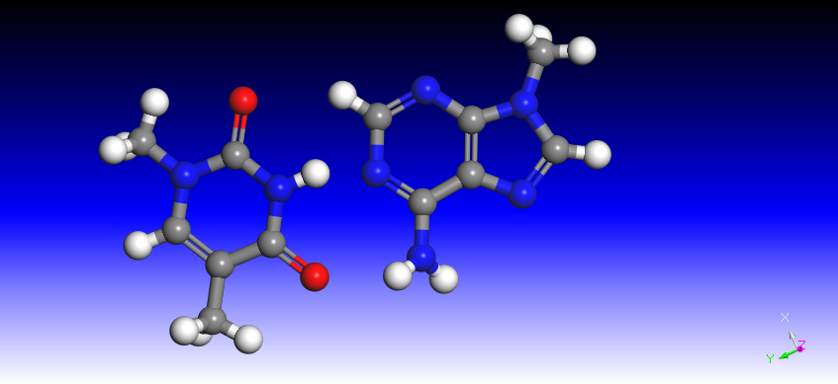
\includegraphics[width=0.7\linewidth]{AT}
	\caption{Hydrogen bonds between AT}
	\label{fig:6}
\end{figure}
\begin{figure}[H]
	\centering
	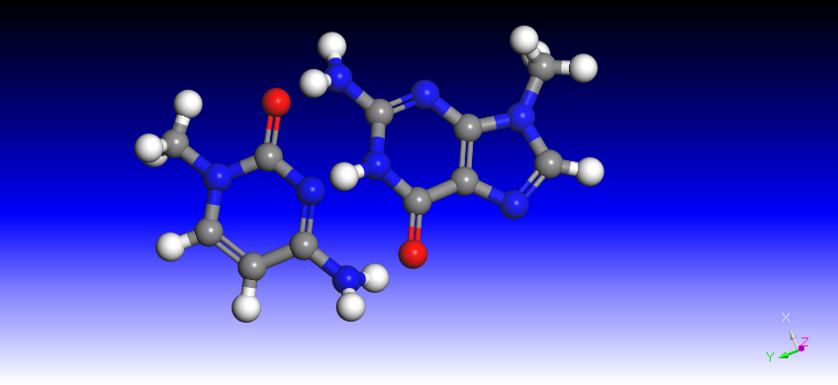
\includegraphics[width=0.7\linewidth]{CG}
	\caption{Hydrogen bonds between CG}
	\label{fig:7}
\end{figure}

The kinetic model sets up a framework to build the relationship between binding probability and the numbers of nucleotide matches and mismatches. In consideration of this problem more carefully, the binding probability becomes equal to the analysis of energy change, because we know the binding energy of A/T and C/G is different due to the different hydrogen bonds between them (figure \ref{fig:6} and \ref{fig:7}), and the energy decrease in C/G is approximately 1.5 folds as A/T. Similarly, the mismatch has more types of variance because the sizes of nucleotides are various. Hence, the types of the mismatched base pair are classified by group volume, i.e., two pyrimidines (such as C/T, “Large”), pyrimidine and purine (such as C/A, “Medium”), two purine (such as G/T, “Small”). Hence, the probability can be calculated using the following equation:
\begin{equation}
P_{bind}=\frac{1}{1+e^{-n_1\Delta_{A/T}-n_2\Delta_{C/G}+n_3\Delta_{L}+n_4\Delta_{M}+n_5\Delta_{S}}}
\end{equation}

\subsection{Parameter Optimization}
From the kinetic model, we can get an output, which is the binding probability. It needs to be noticed that the parameters we choose should make results well discriminated, because in a cleavage experiment, we only have two outcomes, successful(1) and unsuccessful(0). 

To make our predictions from the model more approximate to experiment(facts), we set a regression module and implement parameter optimization. Here, the method we choose is stochastic gradient descent (SGD) and cross entropy. Their principles can be concluded as follows:
\begin{equation}
\theta  = \theta  - \eta {\nabla _\theta }J({x^{(i)}},{y^{(i)}},\theta )
\end{equation}
\begin{equation}
loss = \sum\limits_i {{y_i}\ln {y_i}}
\end{equation}
where $\theta$ means the parameter array and J means the loss function. 

Considering the difficulty in gradient calculation, we substitute the differential term with a difference term to accelerate operating speed.\par
\begin{equation}
\frac{{dy}}{{dx}} \approx \frac{{\Delta y}}{{\Delta x}}{\rm{ = }}\frac{{y(x + \delta x) - y(x)}}{{\delta x}}
\end{equation}

By using this simple method, our model can be more vibrant and more reliable with the ability of updating using newest data.

\subsection{Generating sgRNA Candidates}
Meanwhile, we designed a program to generate all the sgRNA candidates for a target gene, and combined with the previous model, we can compare and rank all the candidates.

The principle of the program  is very simple. We use PAM as the input and collect the arrays with a certain length which contain the same beginning code as PAM.

